\documentclass{article}
\usepackage[utf8]{inputenc}
\usepackage{graphicx}
\usepackage{fancyhdr}
\usepackage{listings}
\usepackage{color}
\usepackage{hyperref}
\usepackage{amsmath}
\usepackage{amssymb}
\usepackage{subcaption}
\usepackage{parcolumns}
\usepackage[total={6in, 9in}]{geometry}



\graphicspath{ {images/} }

\pagestyle{fancy}



\title{%
    Server Software \\
    \vspace{0.4cm}
    \large Lecture Notes
}

\author{jerakrs}
\date{February 2018}


\begin{document}

\maketitle

\begin{abstract}
    This document is the lecture note of \textit{Server Software}. The course code is \textit{COMSM2001} and the unit director is \textit{Steve Gregory}.
\end{abstract}


\section{Introduction}

\textbf{Server} is a process running in a concurrent or distributed system providing a service to client processes. While \textbf{Client-server paradigm}

\begin{itemize}
    \item provides access to service or data available at one place.
    \item provides access to service that users cannot access directly.
    \item but efficiency can be problem.
    \item but other paradigms can be more natural.
\end{itemize}

\subsection{Concurrent, Parallel and Distributed}

\begin{itemize}
    \item Server is usually part of a distributed system.
    \item Server itself may be parallel, for speed and/or reliability.
    \item Server is usually concurrent, to handle multiple clients.
\end{itemize}

\begin{figure}
    \centering
    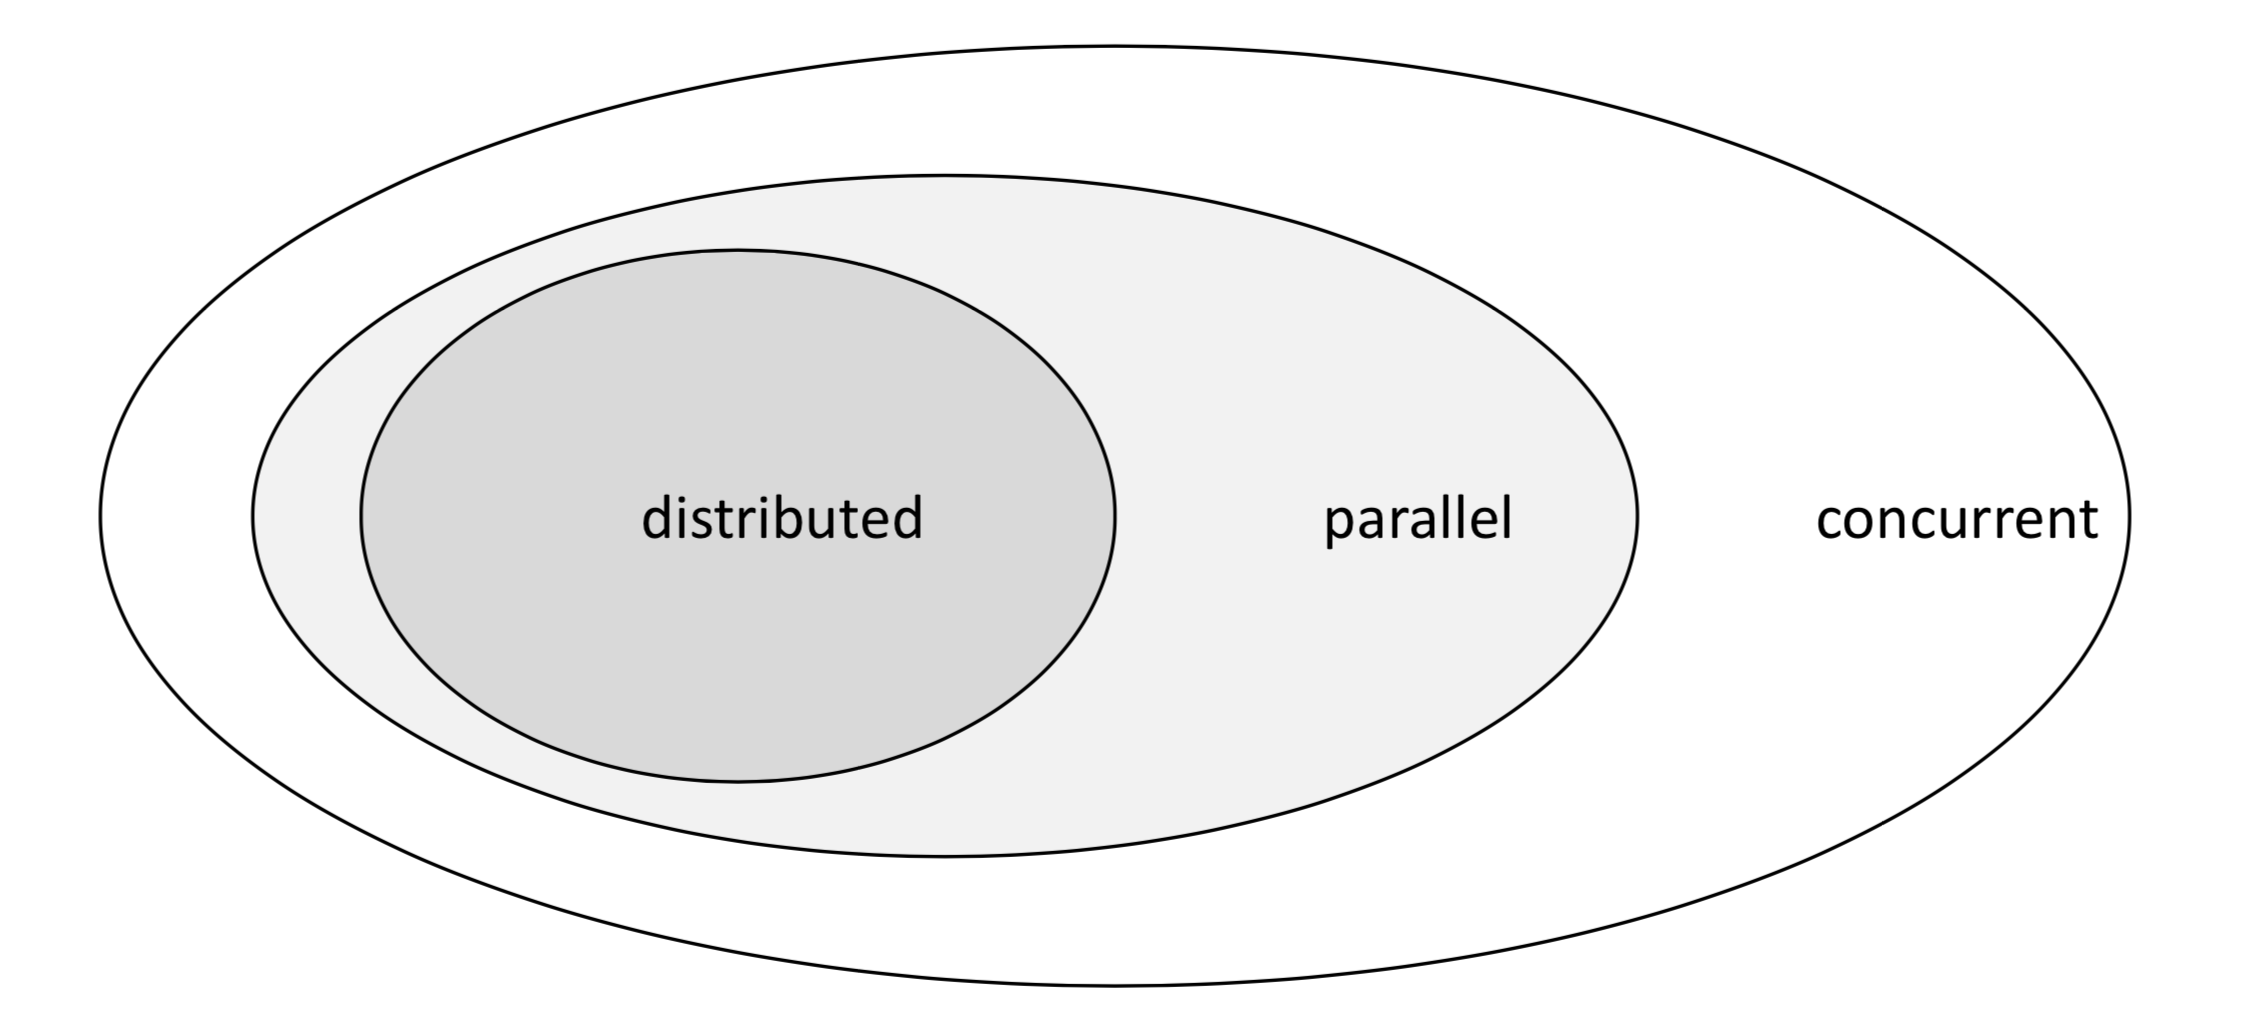
\includegraphics[scale=0.12]{images/relationship.png}
    \caption{Relationship of concurrent, parallel and distributed}
    \label{fig:my_label}
\end{figure}


\subsection{Synchronous vs. Asynchronous}

\begin{itemize}
    \item Synchronous
    \begin{itemize}
        \item need to wait until it can start.
        \item caller blocked until the operation finishes.
    \end{itemize}
    \item Asynchronous
    \begin{itemize}
        \item can test if something is ready.
        \item concurrency – run “in background”
    \end{itemize}
\end{itemize}



\section{C programming}

\subsection{The Error Checking of File Operation }

\begin{lstlisting}[
    frame=shadowbox,
    numbers=left,
    caption=Example of File Operation]
FILE* file = fopen("name", "r");
if (file == NULL) {
    printf("Error opening file: %s\n", strerror(errno));
    exit(EXIT_FAILURE);
}

char buffer[80];
fscanf(file, "%79s", buffer);

if (ferror(file)) {
    printf("Error reading file: %s\n", strerror(errno));
    exit(EXIT_FAILURE);
} else {
    printf("Hello %s\n", buffer);
}

if (fclose(file) != 0) {
    printf("Error closing file: %s\n", strerror(errno));
    exit(EXIT_FAILURE);
}

exit(EXIT_SUCCESS);
\end{lstlisting}

There are four common problems:
\begin{itemize}
    \item fail to open file
    \item buffer overflow
    \item fail to read/write file
    \item forget to close file or fail to close file
\end{itemize}

\textbf{Library}:

\begin{itemize}
    \item \textbf{int errno} (\textit{errno.h}) will set/cleared by C library functions to indicate an error.
    \item \textbf{char* strerror(int errno)} (\textit{string.h}) will return a pointer to a string describing the error code.
    \item \textbf{void exit(int exitno)} (\textit{stdlib.h}) will exit the program, while $0$ = success, $!0$ = error. And exit(i) is the same as “return i” in main().
    \item \textbf{int feof(FILE* file)} (\textit{stdio.h}) will check for end-of file, while $ret = 0$ means file is unfinished, $ret = !0$ means file is finished.
    \item \textbf{int ferror(FILE* file)} (\textit{stdio.h}) will check for errors, while $ret = 0$ means it has no error, $ret = !0$ means it has error.
\end{itemize}


\subsection{The Error Checking of Heap Memory}

\begin{lstlisting}[
    frame=shadowbox,
    numbers=left,
    caption=Example of Heap Memory]
buffer = malloc(BUF_SIZE);
if (buffer == NULL) {
    printf("Error to apply memory.\n");
    exit(EXIT_FAILURE);
}

int err = do_work(buffer);
if (err) {
    printf("Error to use memory.\n");
    exit(EXIT_FAILURE);
}

free(buffer);

exit(EXIT_SUCCESS);
\end{lstlisting}

There are three common problems:
\begin{itemize}
    \item fail to apply memory.
    \item error in using memory.
    \item forget to free memory.
\end{itemize}

\textbf{Library}

\begin{itemize}
    \item \textbf{void *malloc(int bytes)} (\textit{stdlib.h}) allocates the specified number of bytes, while $ret = NULL$ means fail, $ret = !NULL$ means success.
    \item \textbf{void free(void *ptr)} (\textit{stdlib.h}) deallocates the memory previously allocated.
\end{itemize}



\section{Processes}

Process is the execution of a program. A program can be run as many processes and a program may comprise many processes. Each process has an id, the command \textit{ps [-A]} can show them.

\textbf{Concurrency}: At regular intervals, the processor receives a timer interrupt and switches to the operating system. The process has three states: running, ready, blocked. The OS maintains a list of ready processes – which one gets to run next is determined by a scheduling policy. There is also a list for blocked processes.

\subsection{Multiprocess Error Checking}

\begin{lstlisting}[
    frame=shadowbox,
    numbers=left,
    caption=The Example of Multiprocess]
int pid = fork();

if (pid == 0) {
    printf("I'm the child\n");
    exit(EXIT_SUCCESS);
    
} else if (pid > 0) {
    printf("I'm the paraent\n");

    int result;
    int err = waitpid(pid, &result, 0);
    if (err == pid) {
        printf("Child done-returned %i.\n", result);
    } else {
        printf("Error.");
    }
    
} else {
    printf("Fork failed!\n");
    exit(EXIT_FAILURE);
}

return EXIT_SUCCESS;
\end{lstlisting}

\textbf{Library}:

\begin{itemize}
    \item \textbf{int fork(void)} (\textit{unistd.h}) will create a clone of the current process, while $ret = -1$ means create child process fail, $ret = 0$ means this is child process and $ret = PID$ means success.
    \item \textbf{int kill(int pid, int sig)} (\textit{signal.h}) will send a signal to a process or a group of processes specified by pid.
    \begin{itemize}
        \item kill(PID) sends a signal to another process, usually to kill it.
        \item kill(-1) sends a signal to all processes.
    \end{itemize}
    \item \textbf{int waitpid(int pid, int *status, int options)} (\textit{sys/types.h}) will wait for child process with identifier pid to terminate and write the return value into status.
    \begin{itemize}
        \item $pid=-1$ waits for any (one) child.
        \item $options=0$ normally.
        \item $option=WNOHANG$ the process will test if there is currently a finished child.
    \end{itemize}
\end{itemize}



\section{I/O}

C/POSIX processes interact with “files” through file descriptors. \textbf{Everything is a file}: file I/O can be used for pipes, sockets, raw devices

\subsection{stdio}

The three input/output (I/O) connections are called standard input (stdin 0), standard output (stdout 1) and standard error (stderr 2).

\begin{figure}[h]
    \centering
    \begin{subfigure}{0.45\textwidth}
        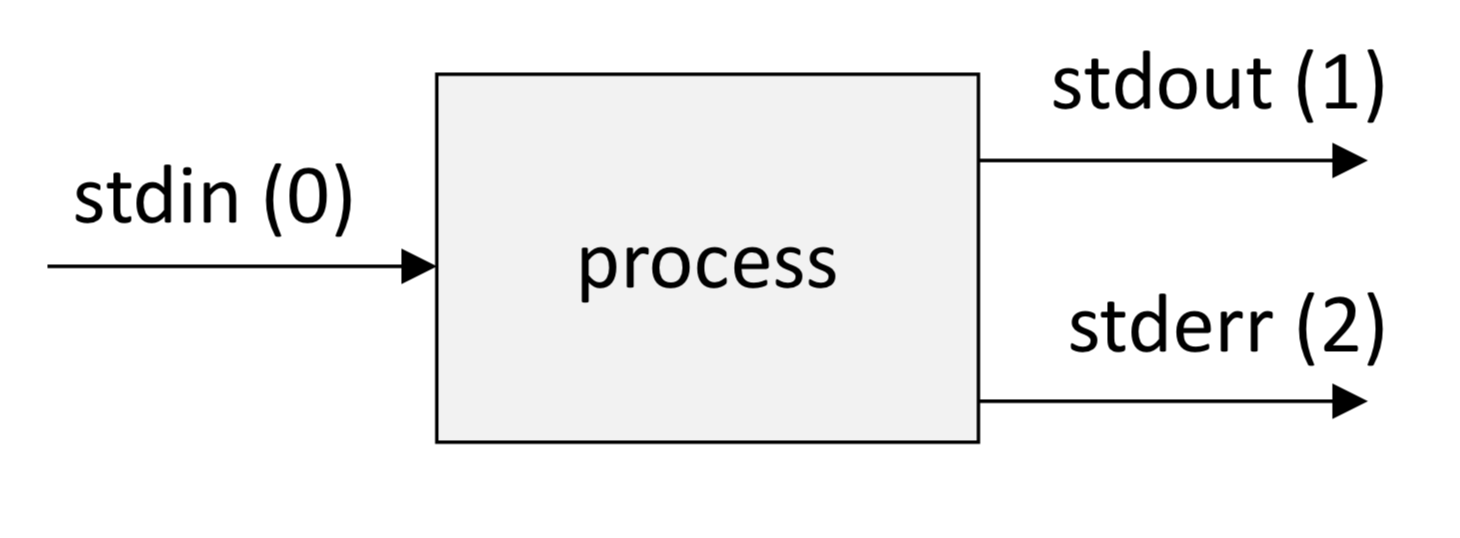
\includegraphics[scale=0.2]{images/stdio.png}
        \caption{stdio}
        \label{fig:my_label}
    \end{subfigure}
    \begin{subfigure}{0.45\textwidth}
        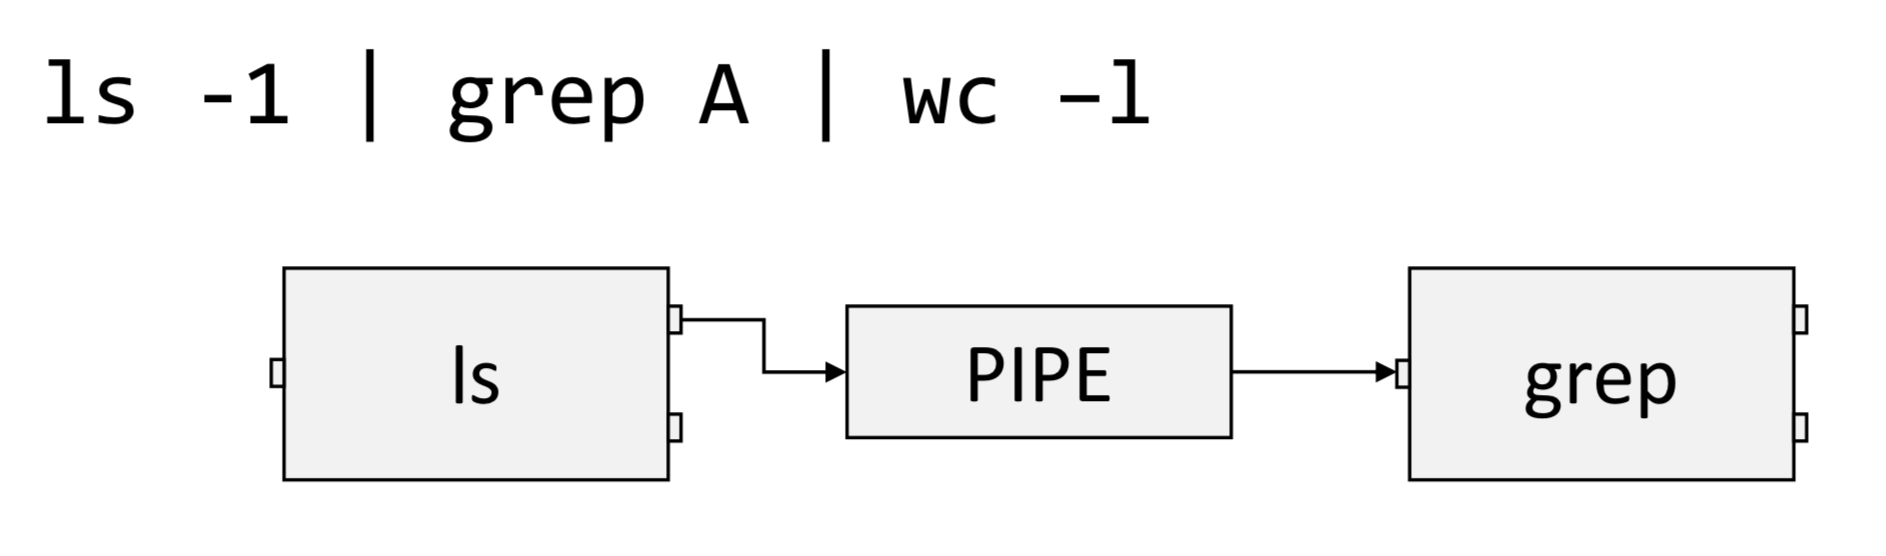
\includegraphics[scale=0.2]{images/pipe.png}
        \caption{pipe}
        \label{fig:my_label}
    \end{subfigure}
\end{figure}

\subsection{pipes}

A pipe is a “special file”: its contents do not exist on any disk.



\section{Threads}

A thread is a “lightweight process”.

\subsection{Processes Vs Threads}

\begin{itemize}
    \item Processes
    \begin{itemize}
        \item Multiple simultaneous programs.
        \item Independent memory space.
        \item Independent open file descriptors.
        \item A process is a container for threads.
    \end{itemize}
    \item Threads
    \begin{itemize}
        \item Multiple simultaneous functions.
        \item Shared memory space.
        \item Shared open file descriptors.
        \item One copy of the heap.
        \item One copy of the code.
        \item Multiple stacks.
    \end{itemize}
\end{itemize}

\subsection{Race Conditions}

\begin{figure}[h]
    \centering
    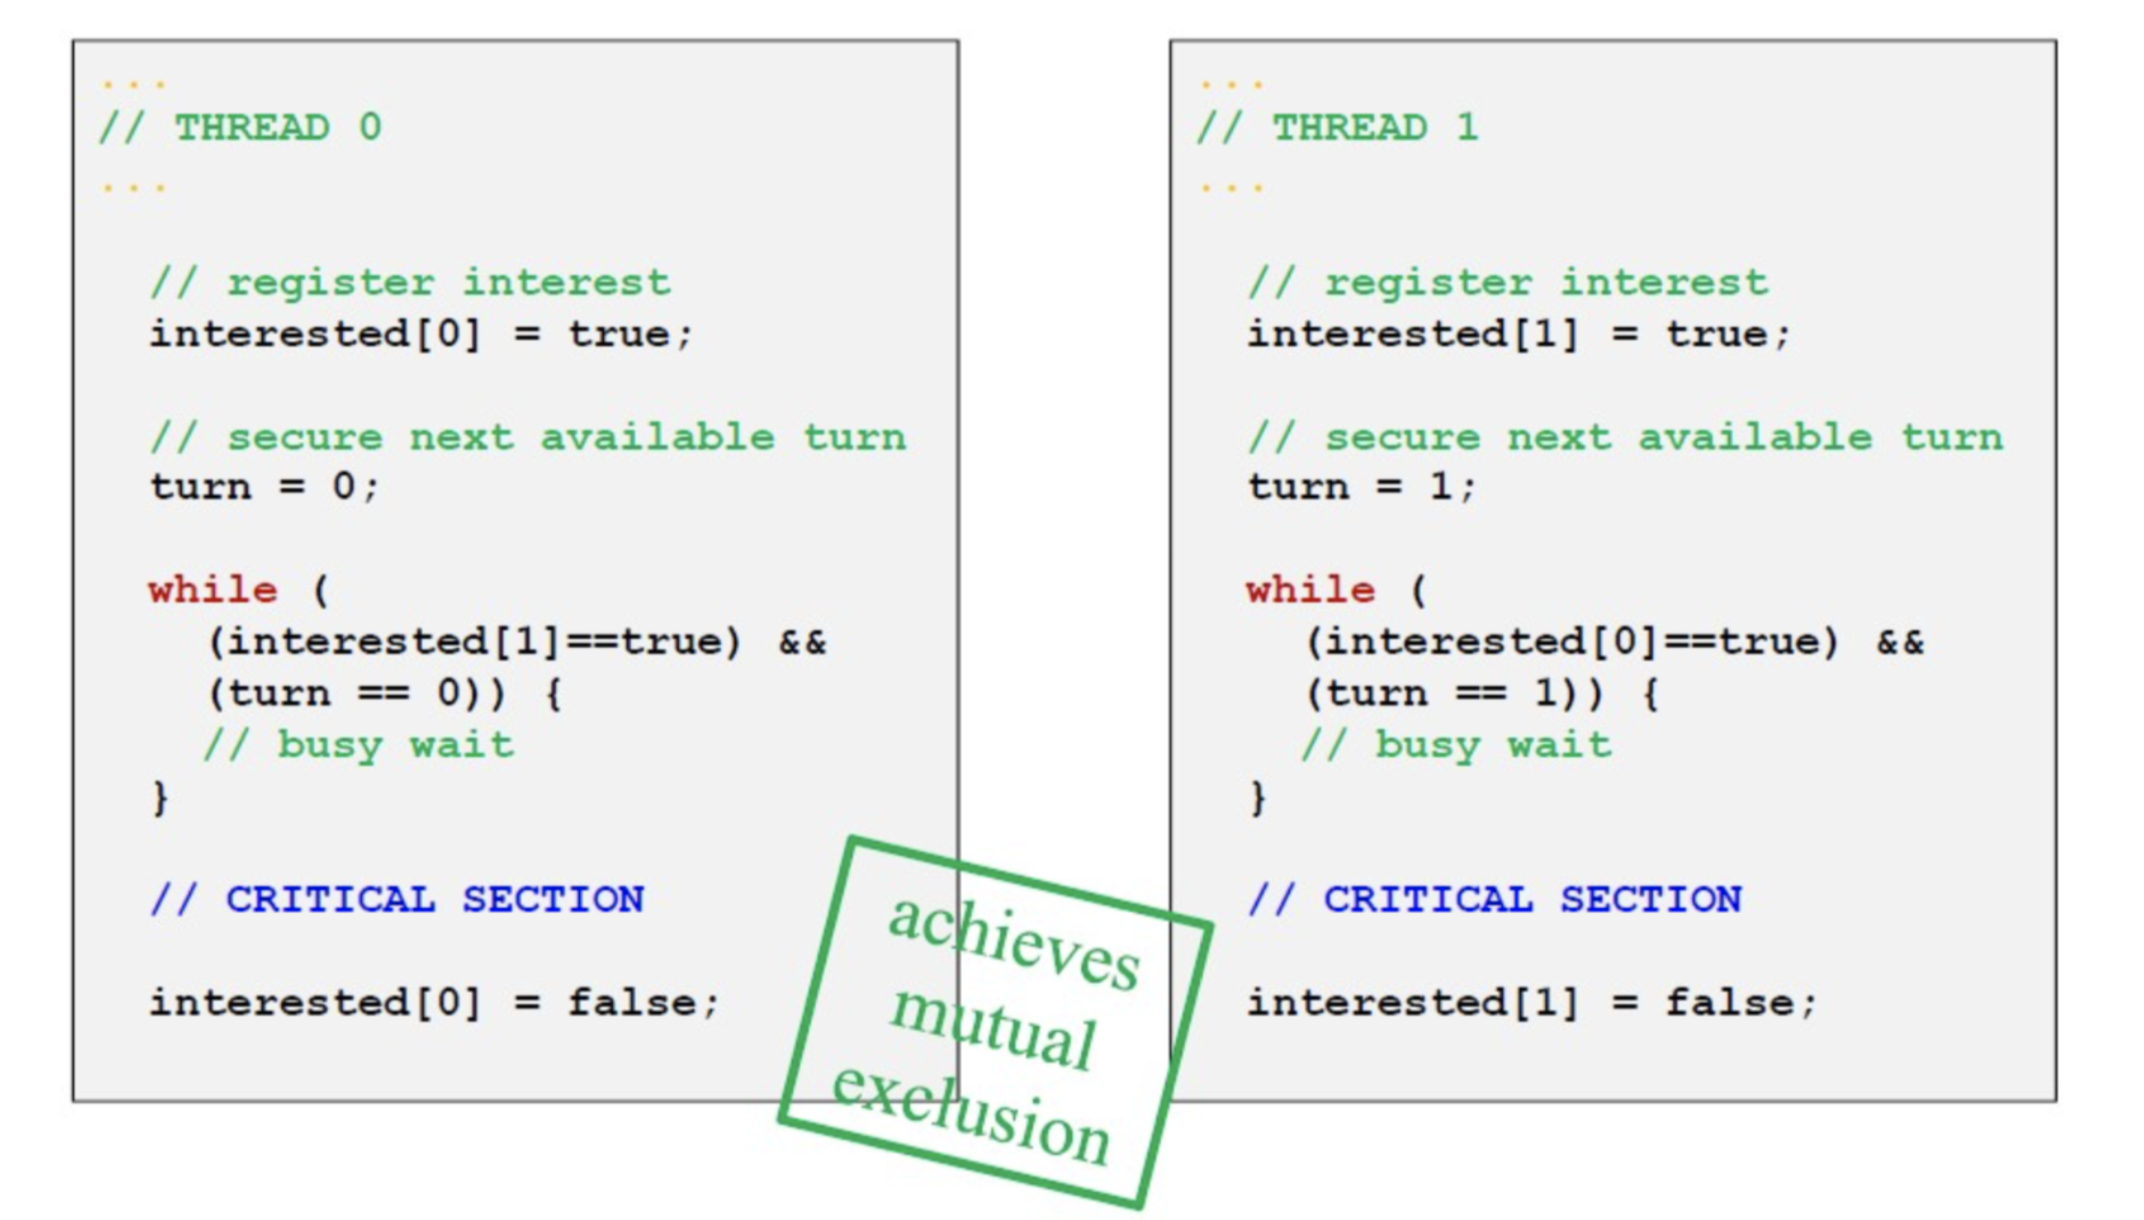
\includegraphics[scale=0.3]{images/peterson.png}
    \caption{Peterson’s Algorithm}
    \label{fig:my_label}
\end{figure}


\subsection{pthread: POSIX threads}

\textbf{thread\_creation}

\begin{lstlisting}
int pthread_create(
    pthread_t *tidp, const pthread_attr_t *attr,
    (void*)(*start_rtn)(void*), void *arg)
\end{lstlisting}

\begin{itemize}
    \item the first argument is a pointer to the pthread\_t.
    \item the third argument is a function, the fourth its argument.
    \item return an int which is 0 for success and the error code otherwise.
\end{itemize}

\noindent \textbf{thread\_join}

\begin{lstlisting}
int pthread_join(pthread_t thread, void **retval);
\end{lstlisting}

\begin{itemize}
    \item pthread\_join blocks if the thread is still alive.
\end{itemize}



\section{Mutual Exclusion}

\textbf{Mutual Exclusion} (mutex) is a property of concurrency control, which is instituted for the purpose of preventing race conditions. The header file is \textit{pthread.h}

\begin{lstlisting}[
    frame=shadowbox,
    numbers=left,
    caption=mutex]
// no need to destory
pthread_mutex_t mut = PTHREAD_MUTEX_INITIALIZER;

// 0: success, !0: fail.
pthread_mutex_init(&lock, NULL);

int pthread_mutex_lock(pthread_mutex_t*);
int pthread_mutex_unlock(pthread_mutex_t*);

// non-blocking function
// 0: mutex was free, !0: mutex is locked
int pthread_mutex_trylock(pthread_mutex_t*);

int pthread_mutex_destroy(pthread_mutex_t*);
\end{lstlisting}



\section{Condition Variables}

\textbf{Problem}: Two variables $x, y$, two threads, the first thread will do some operations when $x > y$, the second thread will swap $x$ and $y$ when $x \leq y$.

\subsection{Busy Waiting}

\begin{minipage}{\textwidth}

\begin{parcolumns}{2}
\colchunk{
\begin{lstlisting}[
    frame=tlrb,
    numbers=left,
    caption=Thread 1]
while (!done) {
    LOCK(lock);
    if (x > y) {
        OPERATE x, y;
        done = 1;
    }
    UNLOCK(lock);
}
\end{lstlisting}
}

\colchunk{
\begin{lstlisting}[
    frame=tlrb,
    caption=Thread 2]
while (!done) {
    LOCK(lock);
    if (x <= y) {
        SWAP x, y;
        done = 1;
    }
    UNLOCK(lock);
}
\end{lstlisting}
}

\end{parcolumns}
\end{minipage}

\subsection{Condition Variables}

When a thread needs to wait for something, it goes to sleep. When a thread does something, it will wakes all threads up. Threads that wake up but can’t find anything to do go back to sleep.

\textbf{Basic operations}

\begin{itemize}
    \item wait – go to sleep until someone wakes you up
    \item signal – wake up exactly one sleeper
    \item broadcast – wake up all sleepers
\end{itemize}

\textbf{Library}

\begin{itemize}
    \item \textbf{pthread\_cond\_t condition = PTHREAD\_COND\_INITIALIZER} (\textit{pthread.h}) initialise a static condition variable, which do not need to destroy.
    \item \textbf{int pthread\_cond\_init(*condition, NULL)} (\textit{pthread.h}) initialises a dynamic condition variable specified by \textit{condition} argument, $ret = 0$ means success, $ret != 0$ means error.
    \item \textbf{int pthread\_cond\_destroy(*condition)} (\textit{pthread.h}) destroy a dynamic condition variable specified by \textit{condition} argument, $ret = 0$ means success, $ret != 0$ means error.
    \item \textbf{int pthread\_cond\_wait(*condition, *mutex)} (\textit{pthread.h}) thread go to sleep and unlock the mutex; after weak up, it will reapply the metux.
    \item \textbf{int pthread\_cond\_signal(*condition)} (\textit{pthread.h}) wake exactly one of sleeper.
    \item \textbf{int pthread\_cond\_broadcast(*condition)} (\textit{pthread.h}) wake all sleepers.
\end{itemize}

\begin{minipage}{\textwidth}

\begin{parcolumns}{2}
\colchunk{
\begin{lstlisting}[
    frame=tlrb,
    numbers=left,
    caption=Thread 1]
LOCK(lock);
while (x <= y) {
    WAIT(cond, lock);
}   
OPERATE x, y;
UNLOCK(lock);
\end{lstlisting}
}

\colchunk{
\begin{lstlisting}[
    frame=tlrb,
    caption=Thread 2]
LOCK(lock);
while (x > y) {
    WAIT(cond, lock);
}   
SWAP x, y;
BROADCAST(cond);
UNLOCK(lock);
\end{lstlisting}
}

\end{parcolumns}
\end{minipage}

\textbf{Benefit}: Sleeper will not occupy the CPU resources.




\section{Semaphores}

Semaphores are an alternative to condition variables. They are not part of the pthreads library and which technique to use depends on the application.

A semaphore has a value $\geq 0$. Operations:

\begin{itemize}
    \item post - increase the value by 1 (atomically).
    \item wait – if $> 0$, decrease by 1 (atomically), otherwise wait until this becomes possible.
\end{itemize}

\textbf{Library}

\begin{itemize}
    \item \textbf{sem\_t semaphore} (\textit{semaphore.h})
    \item \textbf{int sem\_init(*sem, pshared, value)} (\textit{semaphore.h}) initialises the unnamed semaphore specified by the \textit{sem} argument, while \textit{pshared} is ignored (usually be zero) and \textit{value} specifies the value to assign to the newly initialised.
    \item \textbf{int sem\_destroy(*sem)} (\textit{semaphore.h}) destroy a semaphore specified by the \textit{sem} argument.
    \item \textbf{int sem\_wait(*sem)} (\textit{semaphore.h}) locks the specified semaphore by performing a semaphore lock operation on that semaphore, $ret = 0$ means success to lock, $ret = -1$ means error and error message will store in \textit{errno}.
    \item \textbf{int sem\_trywait(*sem)} (\textit{semaphore.h}) locks the specified semaphore only if that semaphore is currently not locked.
    \item \textbf{int sem\_post(*sem)} (\textit{semaphore.h}) unlocks the specified semaphore by performing a semaphore unlock operation on that semaphore, $ret = 0$ means success to lock, $ret = -1$ means error and error message will store in \textit{errno}.
\end{itemize}

\begin{lstlisting}[
    frame=shadowbox,
    numbers=left,
    caption=Semaphore]
sem_wait(&semaphore);
printf("Hello from da thread!\n");
sem_post(&semaphore);
\end{lstlisting}



\section{Safety and Liveness}

\subsection{Safety}

\textbf{Program Safety} refers to the threads safety and encapsulates issues.


\textbf{Race Conditions}: In multithreaded applications the programmer often expects a particular ordering of instructions, while the certain programming errors can lead to non-deterministic ordering, causing undesired behavior. The program can use the atomic instructions or lockers to avoid the race conditions. Atomic instructions (\textbf{Atomicity}) are generally available as compiler extensions and may map to hardware instructions. The lockers allow the programmer to control access to blocks of code, such that we can avoid multiple threads touching the same resources.


\textbf{Library Functions}: The programme should also ensure any functions that the program uses are threads safe.


\subsection{Liveness}

Guaranteeing \textbf{liveness} means that all of the threads are able to make forward progress during their execution. It needs to ensure that threads don’t end up waiting on resources that will never be released.


\textbf{Deadlock} occurs because threads will wait indefinitely on locked shared resources. It is a special case of \textbf{Forward Progress Bugs}.



\section{Communication}

\textbf{Communication Methods:}

\begin{itemize}
    \item Shared memory communication.
    \item Message passing.
    \item Asynchronous message passing.
\end{itemize}

\textbf{Distributed systems}

\begin{itemize}
    \item Peer-to-peer communication:
    \begin{figure}[h]
        \centering
        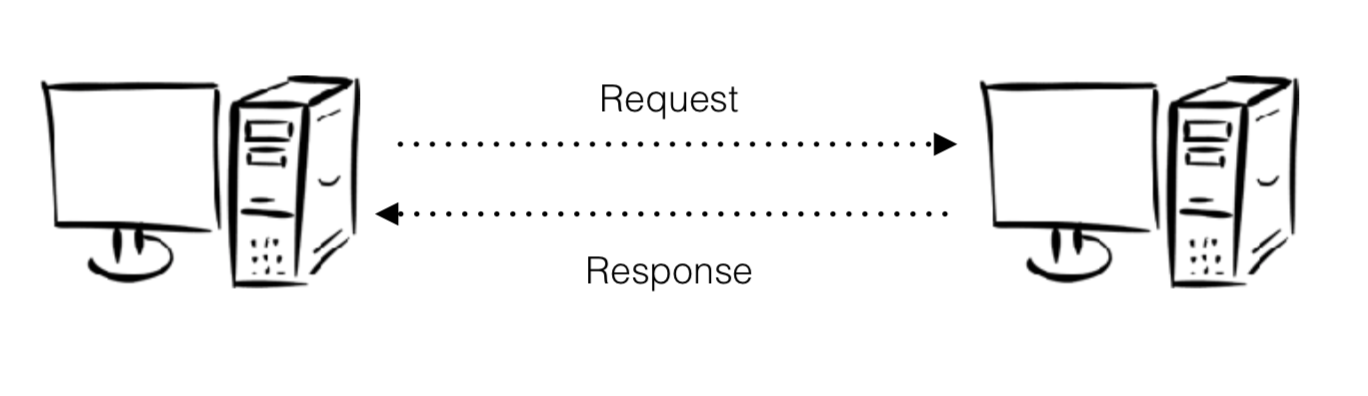
\includegraphics[scale=0.5]{images/peer-to-peer.png}
        \caption{Peer-to-Peer Communication}
        \label{fig:my_label}
    \end{figure}
    \item Server-client communication:
    \begin{figure}[h]
        \centering
        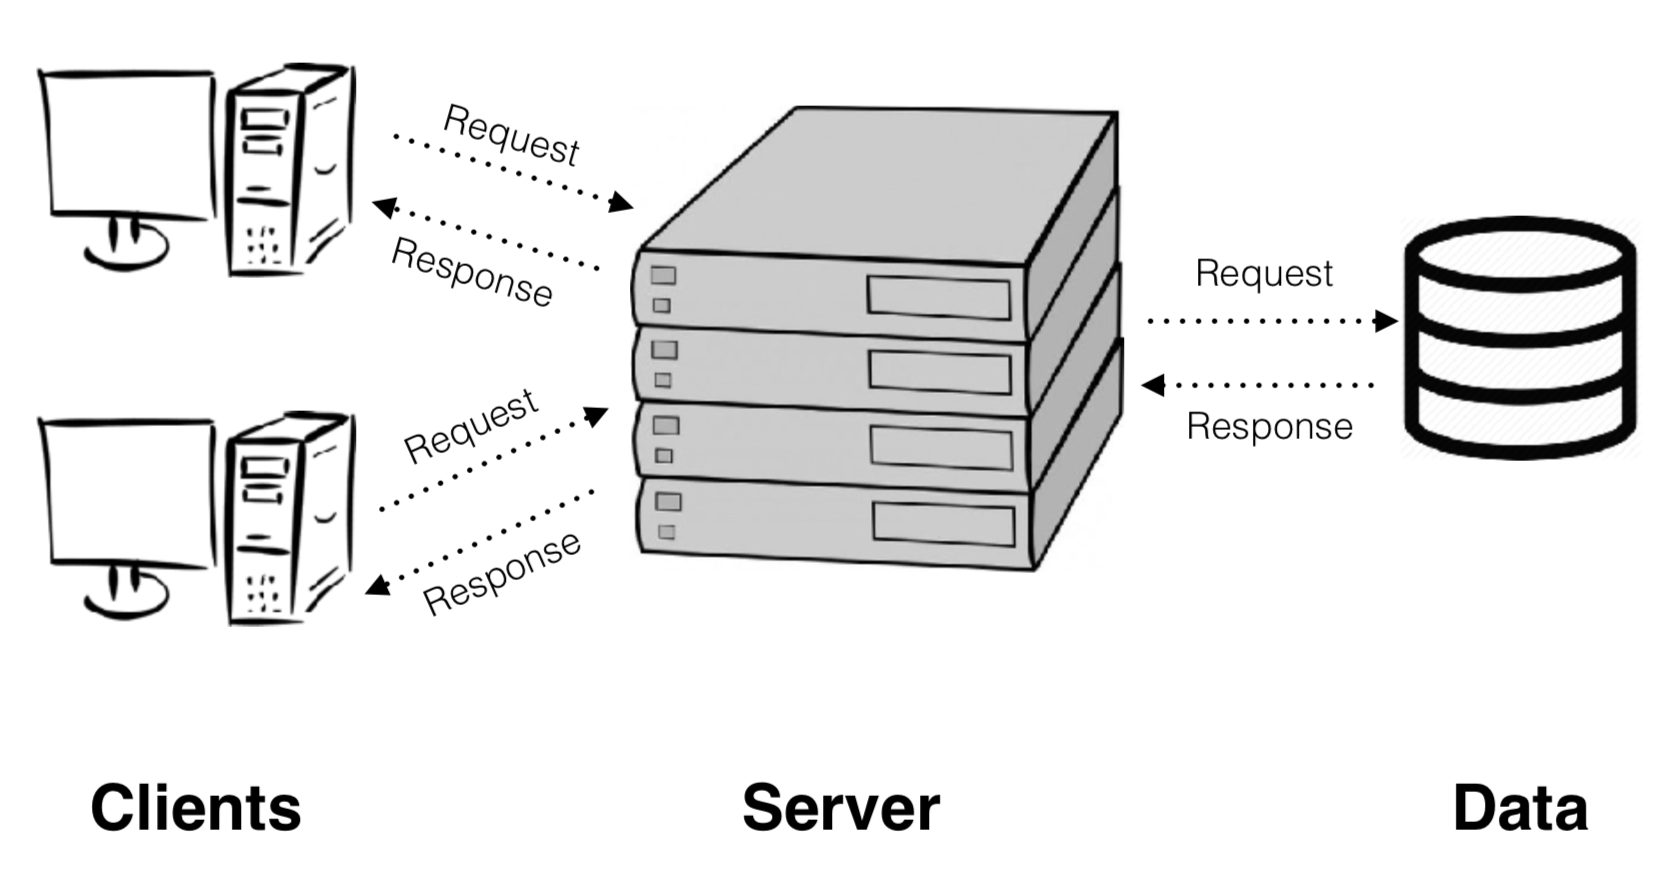
\includegraphics[scale=0.45]{images/server-client.png}
        \caption{Server-Client Communication}
        \label{fig:my_label}
    \end{figure}
\end{itemize}


\section{Sockets}

\subsection{Pipe}

\textbf{1-way communication}

\begin{figure}[h]
    \centering
    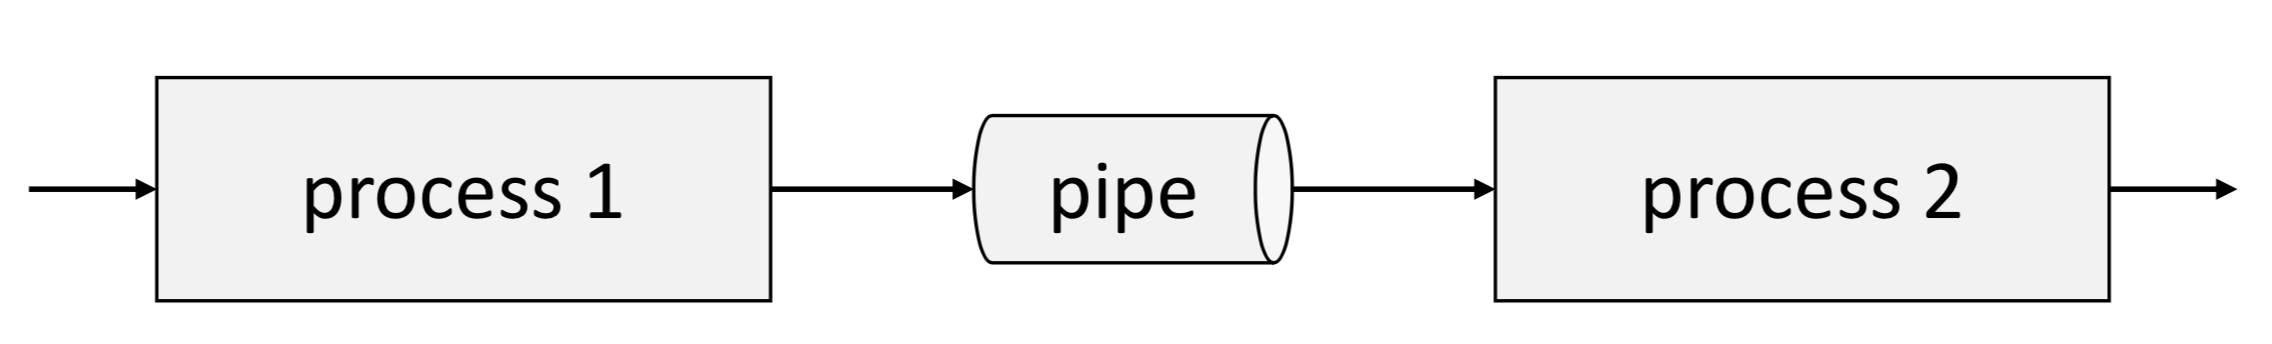
\includegraphics[scale=0.3]{images/pipe-1-way-communication.png}
   \caption{1 Way Communication}
    \label{fig:my_label}
\end{figure}

\textbf{2-way communication}

\begin{figure}[h]
    \centering
    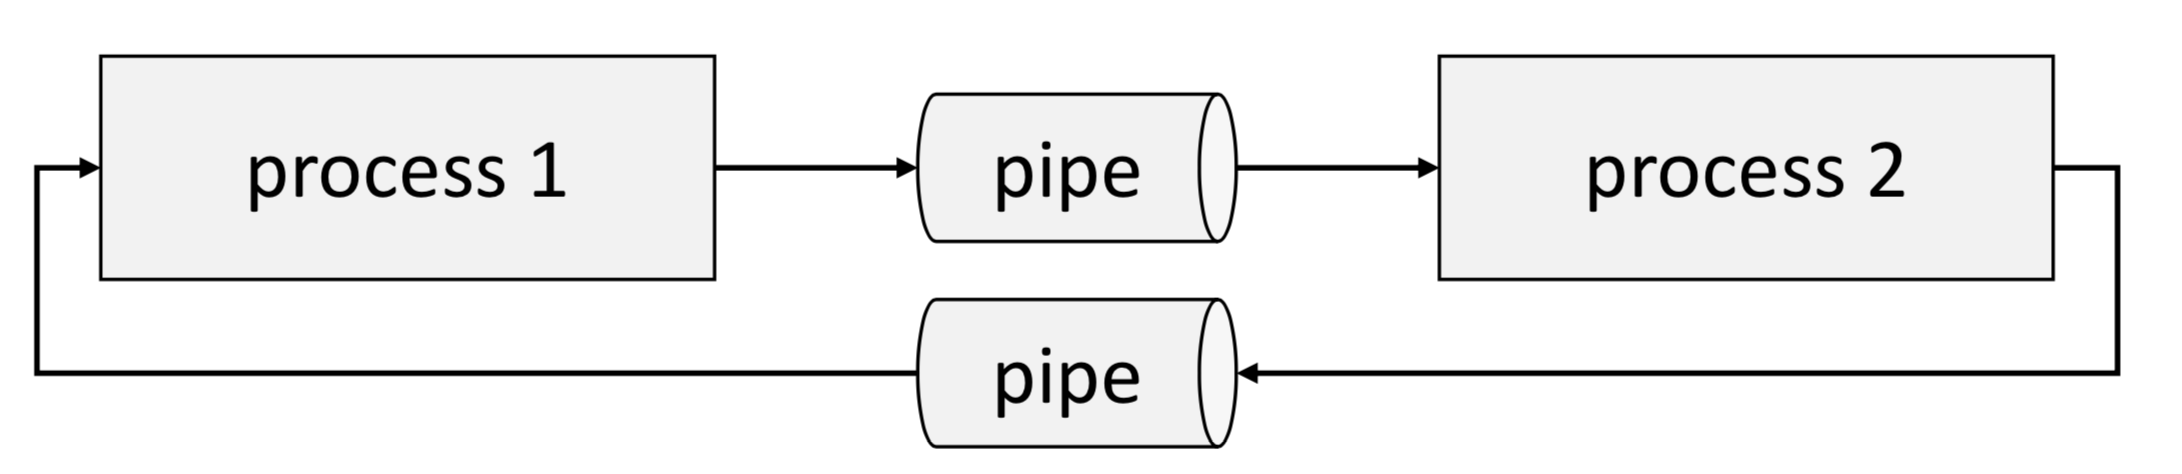
\includegraphics[scale=0.3]{images/pipe-2-way-communication.png}
   \caption{2 Way Communication}
    \label{fig:my_label}
\end{figure}



\subsection{Sockets}

Sockets are one way to implement 2-way channels. The TCP protocol connects sockets on different machines across the internet.

\begin{figure}[h]
    \centering
    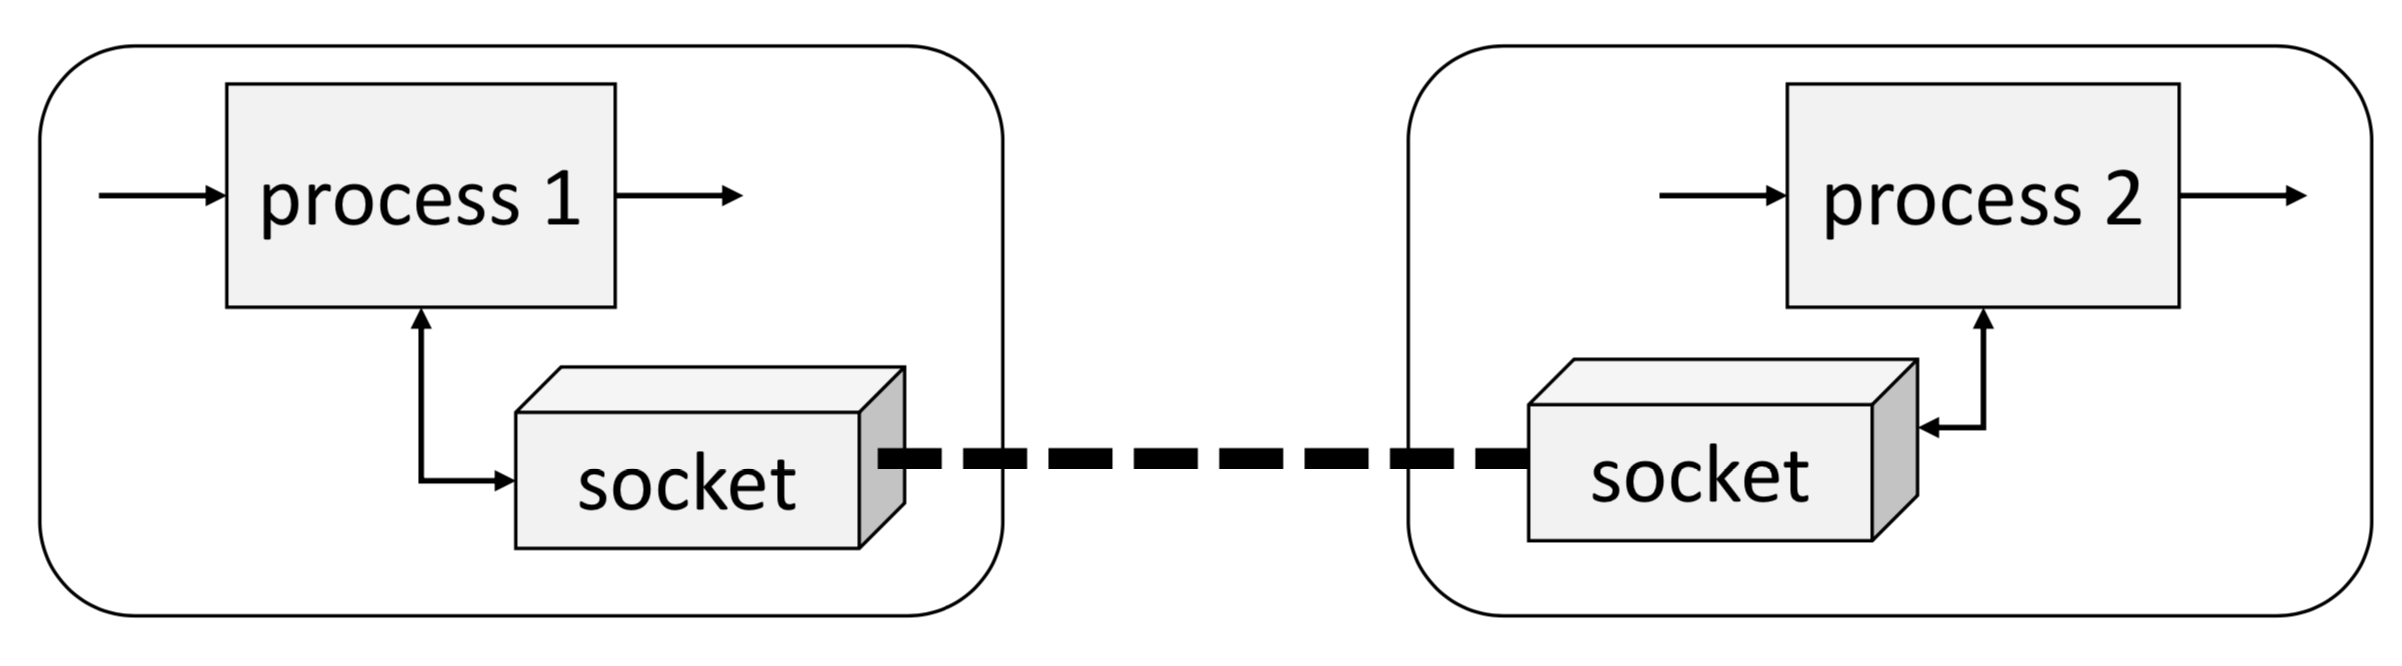
\includegraphics[scale=0.3]{images/tcp-socket.png}
   \caption{TCP socket}
    \label{fig:my_label}
\end{figure}


\textbf{socket states:}

\begin{figure}[h]
    \centering
    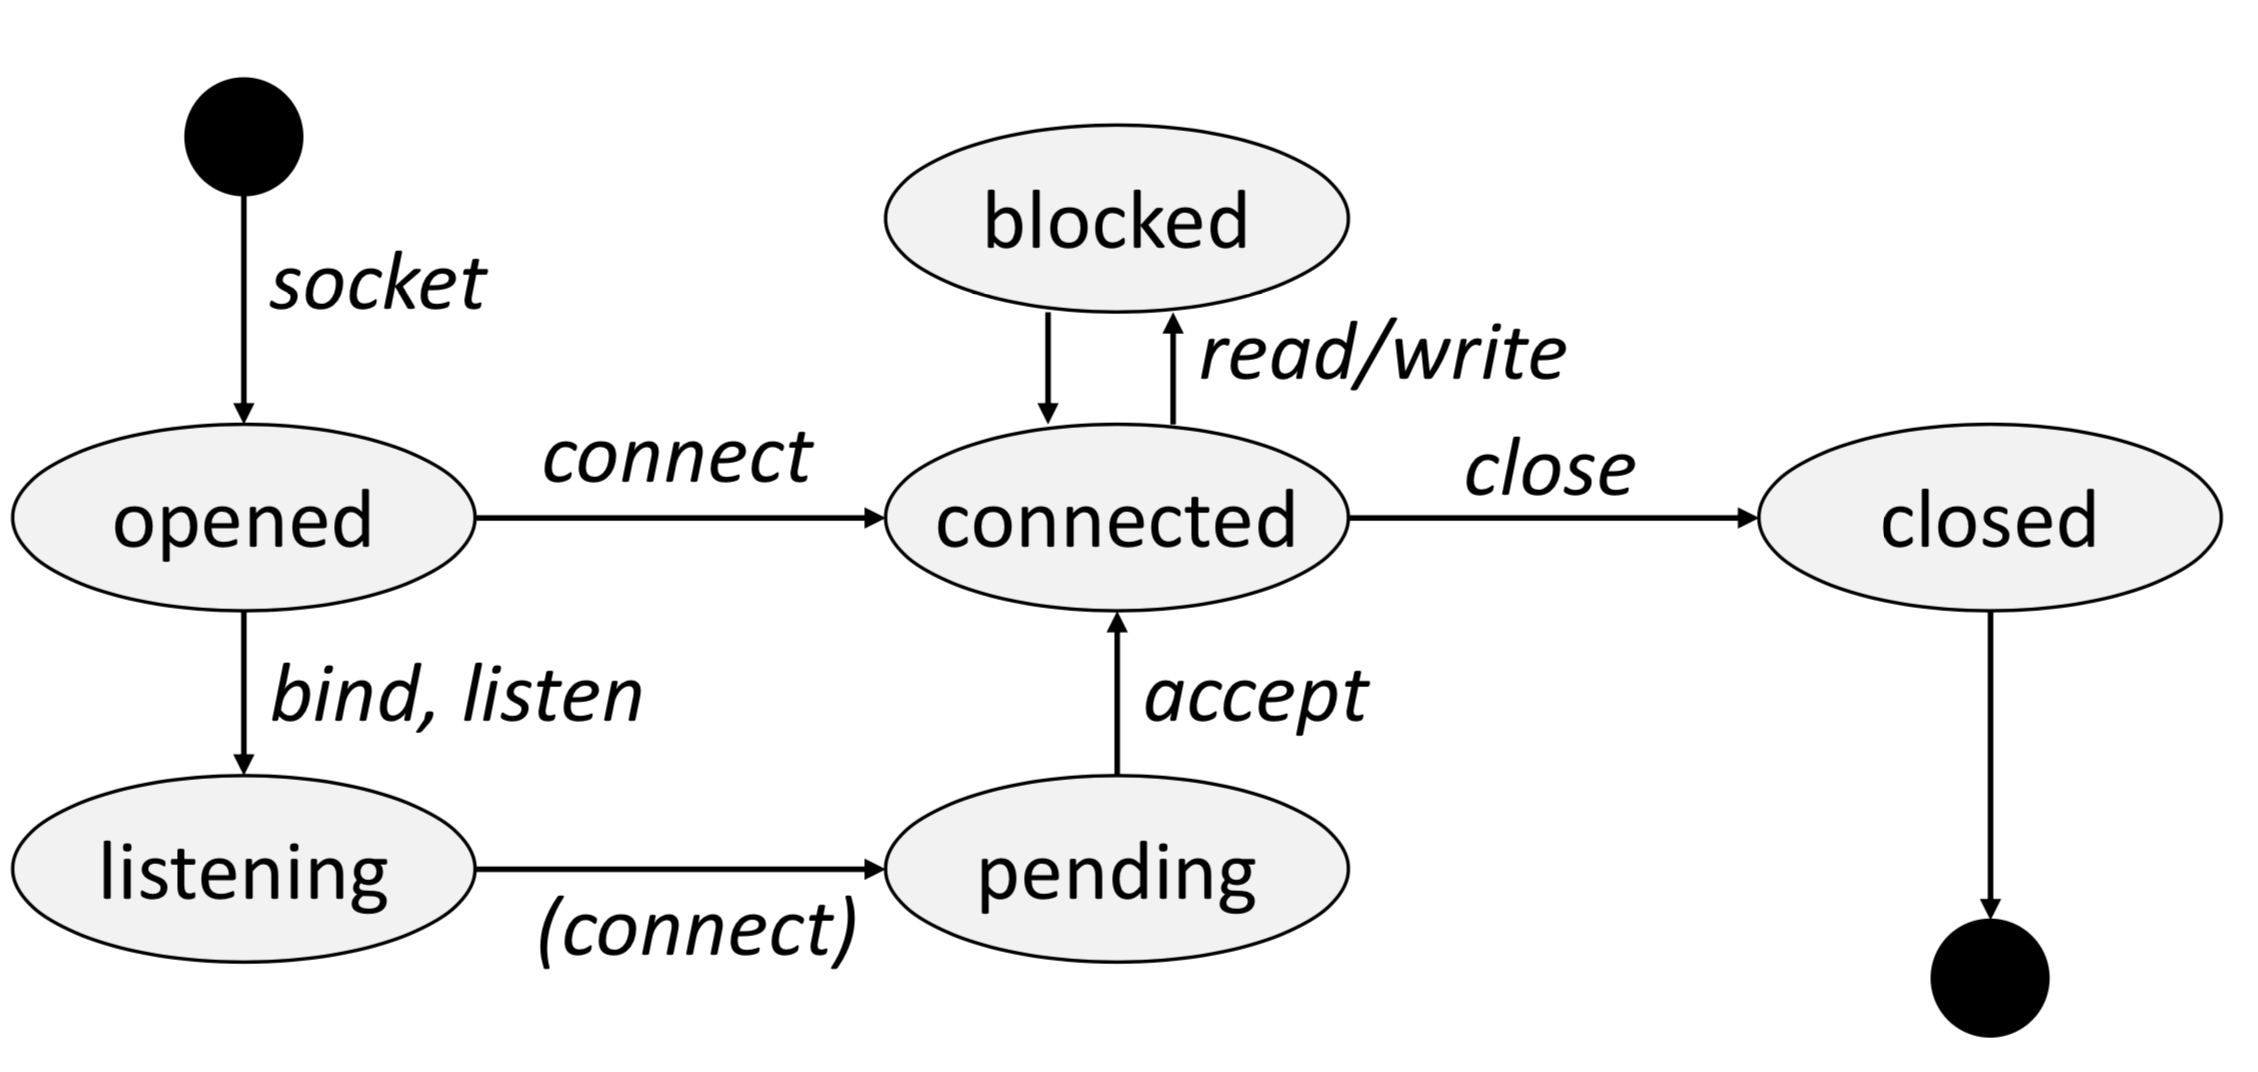
\includegraphics[scale=0.3]{images/socket-states.png}
   \caption{Socket States}
    \label{fig:my_label}
\end{figure}

\textbf{File descriptor}: A file descriptor (fd), like a FILE*, is a way of referring to a file that the operating system has opened


\textbf{Library}

\begin{itemize}
    \item \textbf{int socket(int domain, int type, int protocol)} (\textit{sys/socket.h}) creates a new socket. While \textit{domain=AF\_INET} refers to the IPv4 and \textit{type=SOCK\_STREAM} means using the TCP/IP protocol. The return value is a file descriptor unless fail (\textit{ret=-1}).
    
    \item \textbf{int bind(int fd, struct sockaddr *addr, socklen\_t len)} (\textit{sys/socket.h}) binds the socket to the specific port, while the \textit{fd} refers to the socket and \textit{addr} represents the port.
    
    \item \textbf{int listen(int fd, int backlog)} (\textit{sys/socket.h}) listens the socket to wait the new request.
    
    \item \textbf{int accept(int fd, struct sockaddr *addr, socklen\_t *len)} (\textit{sys/socket.h}) will accept request from the socket, the return value is a new fd for the connection unless fail (\textit{ret=-1}).
    
    \item \textbf{int close(int fd)} (\textit{unistd.h}) close the file descriptor.
    
    \item \textbf{int poll(struct pollfd[] fds, nfds\_t n, int timeout)} (\textit{poll.h}) poll the file descriptors.
\end{itemize}


\section{Transactions}

A transaction is an action or sequence of actions that needs to be performed either fully or not at all. Many database servers offer ACID transactions:

\begin{itemize}
    \item A is for Atomicity.
    \item C is for Consistency.
    \item I is for Isolation.
    \item D is for Durability.
\end{itemize}

\end{document}